\chapter{muEDM entrance detector}
\begin{refsection}

{\itshape
This chapter is an introduction to the muEDM experiment. After describing in some detail the spin dynamics, a brief status on the EDM searches for the different particles will follow.
The description of the muEDM search will follow: starting from the frozen spin technique and outlying the status of the experiment. 
Description of the apparatus, study on the systematics and introduction to the different simulations.}

\section{\gf simulations}
\subsection{Entrance system}
We started with a study on muon interaction with plastic scintillators. This preparative work had two objectives: to make myself reasonably comfortable with \gf (which I never used before) and to take a first step in the direction of an R\&D for the muEDM experiment.

Generic things to check to validate your simulations: 40-50 keV $\rightarrow$ few photoelectrons; if you have more than 10 photo-electrons you are in good shape;

roadmap as of 21 Apr. 2020
\begin{itemize}
\item A cube 1cm x 1cm x 1cm
\begin{itemize}
\item Energy loss per particle
\item Photons on each face of the cube ($\sim 1/6$)
\item Entrance and exit positions
\end{itemize}
\item Start reducing the width (1cm $\rightarrow$ 10 $\mu$m)
\begin{itemize}
\item Enegy deposit: Landau $\rightarrow$ Gauss
\item What happens if momentum: 125 MeV/c $\rightarrow$ 2 MeV/c
\end{itemize}
\item Items down the line, for the 1m scintillator
\begin{itemize}
\item Reflection coefficient
\item Light yield ($\sim 8000\ \gamma/$MeV)
\item $\tau$ ($\sim 2$ns)
\item Attenuation lenght ($\sim 1$m)
\end{itemize}
\end{itemize}

\subsubsection{Rough}
I started saving energy deposited, length in and out points for few geometries (20, 10, 5, 1)x20x20 cm.
What we can see here is that the energy deposited starts looking as a Landau. at the same time is quite interesting to notice that for very high thicknesses (20x20x20 cm) the distribution of the exit point changes substantially. Y and Z are no longer centered around 0 but present two peaks (lateral surfaces) and for the X the number of particles exiting from the same face they entered is quite substantial.

\subsubsection{Refine}
We are interested in 10$\rightarrow$1 x 200 x 200 mm geometries. So let's put something like 2mm and see what happens changing energy and then particle.

\subsubsection{$\mu^+\ 125\rightarrow2$ MeV/c}
\subsubsection{$e^+\ 125\rightarrow2$ MeV/c}

\subsection{Thin scintillators}
\subsection{Telescope and entrance detector}
\section{Beamtime 2021}
During the last part of the 2021, a beam-time was scheduled at PSI to test the pixels telescope and perform some measurements of different degraders.
The overall aim was to develop the necessary data and understanding to write the proposal for the Precursor Experiment of muEDM.\\
\subsection{Describe the apparatus}
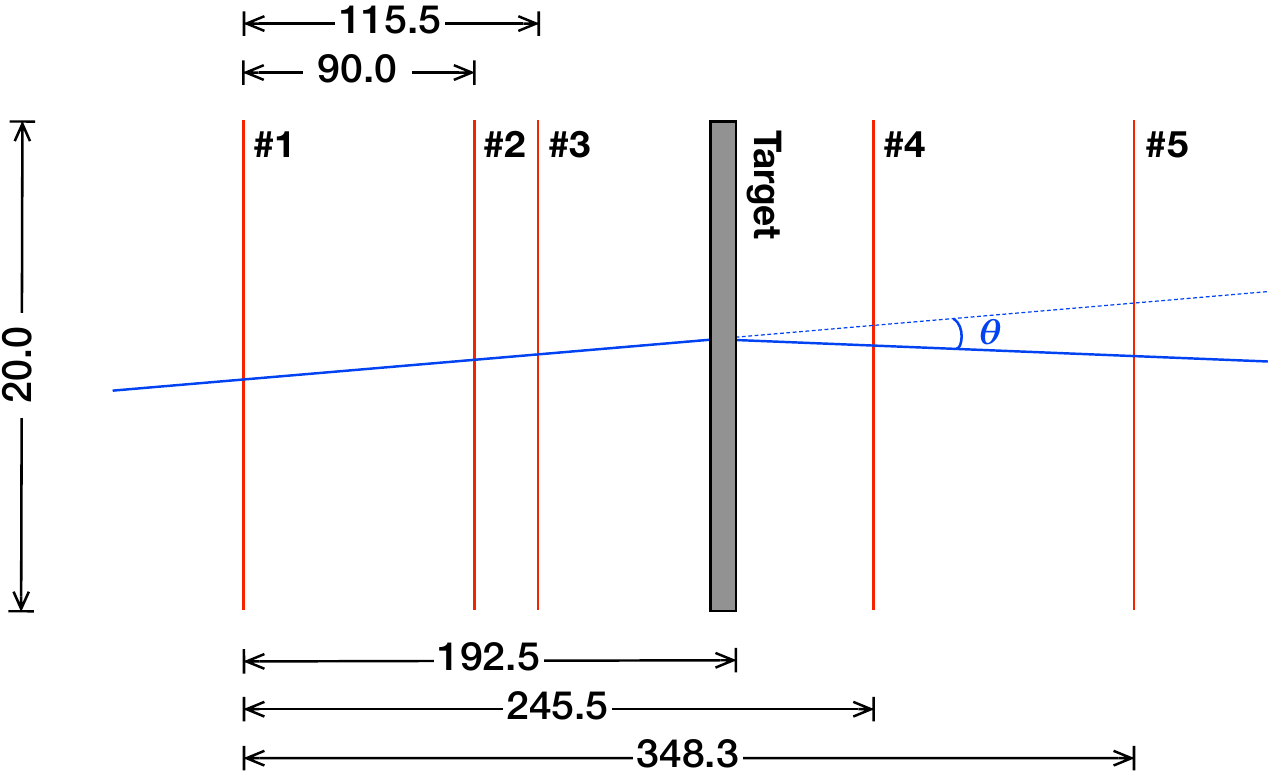
\includegraphics[width=0.8\textwidth]{Figures/muEDM_Dec2021/Positions_Telescope.png}\\
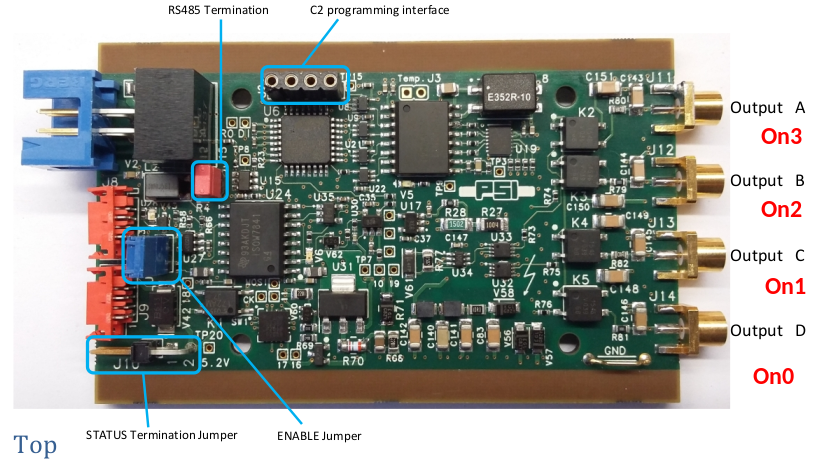
\includegraphics[width=0.8\textwidth]{Figures/muEDM_Dec2021/HV.png}\\
\subsection{Describe the beam}
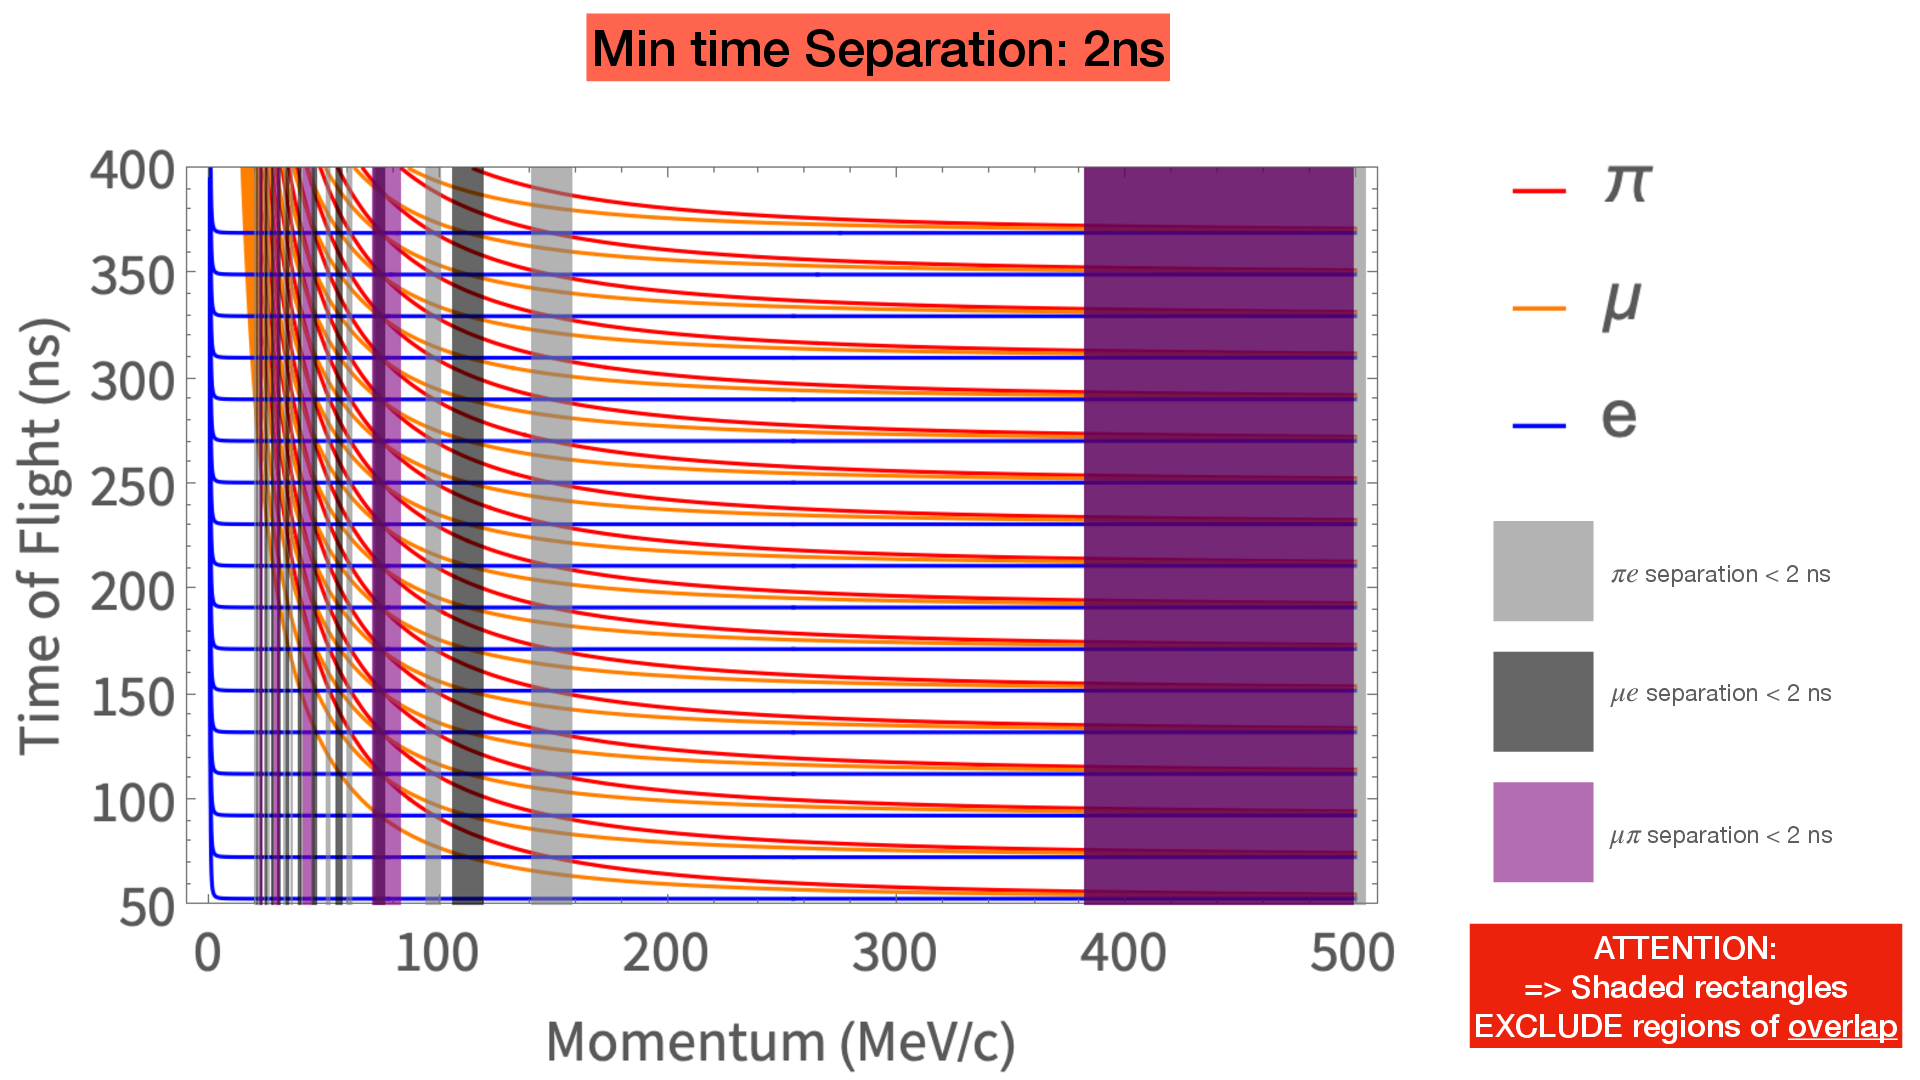
\includegraphics[width=0.8\textwidth]{Figures/muEDM_Dec2021/ToFPlots-0.png}\\

\subsection{Describe the samples}
For our own purpose, we tested mylar samples of variable thickness with different beam settings. These data were taken to crosscheck the simulations and the development of the entrance tagging system for the incoming muons.\\
The data processing was divided in two major steps:
\begin{itemize}
    \item Reconstruction of the pixel information and the creation of .root trees, performed primarily by the Mainz group
    \item Analysis of the TTrees by the different subgroups
\end{itemize}


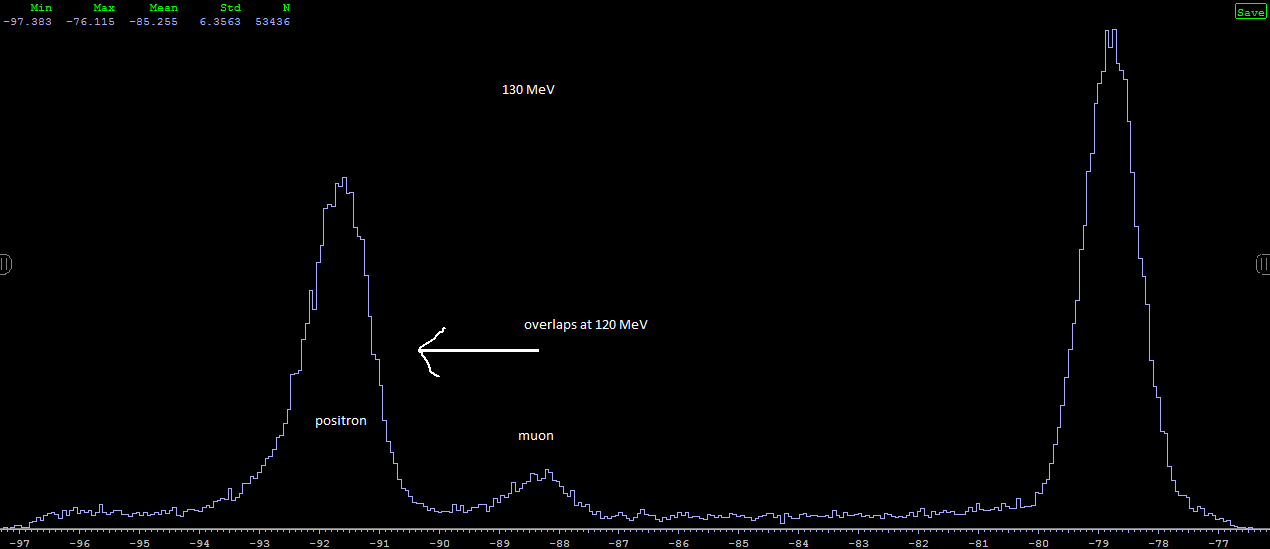
\includegraphics[width=0.8\textwidth]{Figures/muEDM_Dec2021/TOFAllEnergies130.png}\\
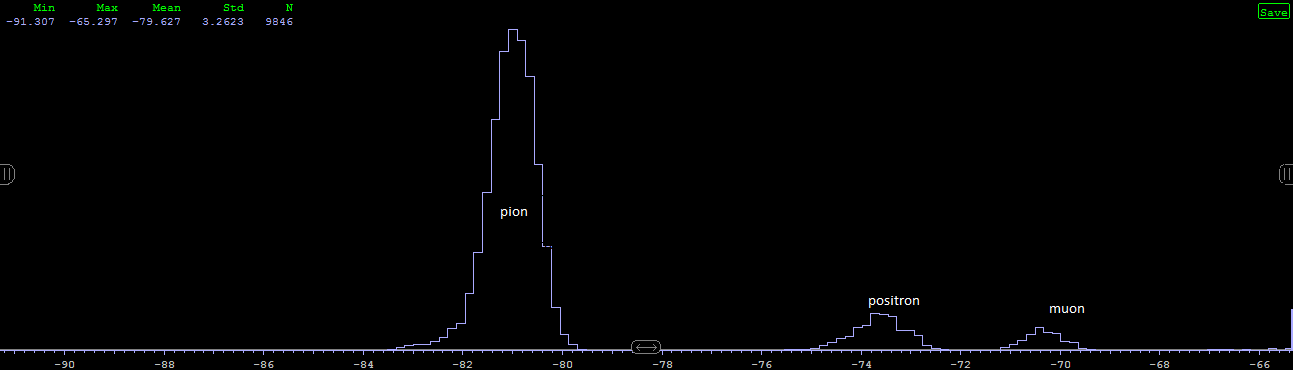
\includegraphics[width=0.8\textwidth]{Figures/muEDM_Dec2021/TOFMediumCut125.png}


\subsection{Data taking}
\subsection{Data analysis}
\section{Beamtime 2022: Telescope and entrance detector}
\subsection{Construction}
\subsection{Data taking}
\subsection{Data analysis}
\section{Beamtime 2023: Multi readout entrance}
\subsection{Data taking}
\subsection{Data analysis}

\section{Conclusions}

\addcontentsline{toc}{chapter}{Bibliography on muEDM entrance detector}
\printbibliography[title=ibliography on muEDM entrance detector]
\end{refsection}